\documentclass[a4paper,10pt]{article}
\usepackage[utf8x]{inputenc}

\usepackage{verse}
\usepackage[slovene]{babel}
\usepackage{graphicx}
\usepackage{hyperref}
\usepackage{amsmath}
\usepackage{amsfonts}
\usepackage{comment}
\usepackage{subfigure}

\usepackage{tikz}
\usetikzlibrary{shapes,arrows}

\tikzstyle{decision} = [diamond, draw, fill=blue!20, 
    text width=4.5em, text badly centered, node distance=3cm, inner sep=0pt]
\tikzstyle{block} = [rectangle, draw, fill=blue!20, 
    text width=5em, text centered, rounded corners, minimum height=4em]
\tikzstyle{line} = [draw, -latex']
\tikzstyle{cloud} = [draw, ellipse,fill=red!20, node distance=3cm,
    minimum height=2em]



\newcommand{\slika}[2]{
\begin{figure}[h]
 \input{#1}
  \caption{#2}
  \label{fig:#1}
\end{figure}
}


%opening
\title{Var\v cni modeli}
\author{Miha \v Can\v cula}

\begin{document}

\maketitle

\section{Splo"sno}

\subsection{Naloga}

Naloge sem re"seval z razcepom matrike $\mathbf{S}$ na singularne vrednosti, tako da sem minimiziral izraz 

\begin{align}
 \chi^2_{red} &= \frac{1}{m-k} \sum_{i=1}^m \left(\frac{(\mathbf{Sa})_i - \mathbf{y}_i}{\sigma_i}\right)^2 \\
  &= \frac{1}{m-k} \left|\mathbf{CSa} - \mathbf{Cy}\right|^2
\end{align}

Tu je $\mathbf{a}$ vektor parametrov, $\mathbf{y}$ vektor meritev odvisne spremenljivke, $\mathbf{S}$ pa modelska matrika ki izmerjene vrednosti neodvisnih spremenljivk povezuje s parametri. $m$ je "stevilo meritev, $k$ pa "stevilo uporabljenih parametrov. Matrika $\mathbf{C}$ je matrika ute"zi, s katero dose"zemo, da imajo posamezne meritve razli"cen vpliv na optimalno vrednost parametrov. V na"sem primeru, ko nimamo korelacij med posameznimi meritvami, je ta matrika diagonalna in podana z $\mathbf{C}_{ii} = \sigma_i^{-1}$. 

Da sem lahko singularne vrednosti matrike $\mathbf{S}$ primerjal med seboj, sem najprej vse spremenljivke normiral, tako da je bil razpon njihovih vrednosti med -1 in 1. Ta interval ima veliko prednost, da ima tudi vsaka potenca spremenljivke vrednosti na tem intervalu. Ker je simetri"cen, se tudi izognemo korelaciji med $x^i$ in $x^{i+1}$, saj je le ena izmed teh dveh funkcij na izbranem intervalu simetri"cna. V obeh primerih sem uporabljal le poten"cne funkcije. 

\subsection{Re"sevanje}

Na matriki $\mathbf{S}$ sem najprej uporabil razcep \texttt{SVD} na dve ortogonalni kvadratni matriki $\mathbf{U}$ in $\mathbf{V}$ ter pravokotno $\mathbf{W}$. 

\begin{align}
 \mathbf{S} &= \mathbf{U W V^T} \\
 \mathbf{a} &= \mathbf{S}^{-1}\mathbf{y} = \mathbf{V W^{-1} U^T y}
\end{align}

Matriki $\mathbf{S}$ in $\mathbf{W}$ nista kvadratni, zato sem uporabil pravilo za izra"cun psevdoinverza. $\mathbf{W}$ je po definiciji razcepa diagonalna, zato jo najprej transponiramo, nato pa popravimo diagonalne elemente
\begin{equation}
 [\mathbf W^{-1}]_{ii} = \left\{ \begin{matrix}
                         1/\mathbf{W_{ii}}, & \mathbf{W_{ii}} > \varepsilon \\
			 0, & \mathrm{sicer}
                        \end{matrix} \right.
\end{equation}

Med ra"cunanjem sem preizku"sal razli"cne vrednosti za $\varepsilon$ in na ta na"cin dobil razli"cno "stevilo uporabljenih parametrov $k$, da bo $\chi^2_{red}$ "cim bli"zje 1. 

To ``bli"zino'' sem definiral kot $b(x) = x + 1/x$, tako da velja $b(x) > 1$ za vsak $x$, ki ni enak 1. Sedaj sem lahko iskal tak"sne vrednosti parametrov, da bo $b(\chi^2_{red})$ "cim manj"si. Hkrati pa sem "si "zelel "cim manj"se "stevilo parametrov, 
zato sem v algoritmu minimiziral $b(x) + \alpha k$. Konstanta $\alpha$ odlo"ca, ali nas zanimajo bolj to"cni ali bolj var"cni modeli. 

\subsection{Napake parametrov}

Napake oz. kovarian"cno matriko koeficientov sem izra"cunal po predpisu in Numerical Recipes

\begin{align}
 \mathbf{Cov} &= \mathbf{V^T W^{-1} V}
\end{align}

"Se posebej so me zanimali diagonalni elementi kovarian"cne matrike, saj sem med seboj primerjal napake in s tem pomembnost parametrov. 

\subsection{Iskanje optimalnega "stevila parametrov}

Optimizacijo sem za"cel z velikim "stevilom testnih funkcij, ki so bile kar prvih nekaj potenc neodvisnih spremenljivk. Po zgornjih formulah sem izra"cunal koeficiente pred temi funkcijami in njihove napake.

\begin{comment}

Nato sem odstranjeval testne funkcije po algoritmu na sliki \ref{fig:alg-izlocanje}. 

\begin{figure}[!h]
\centering
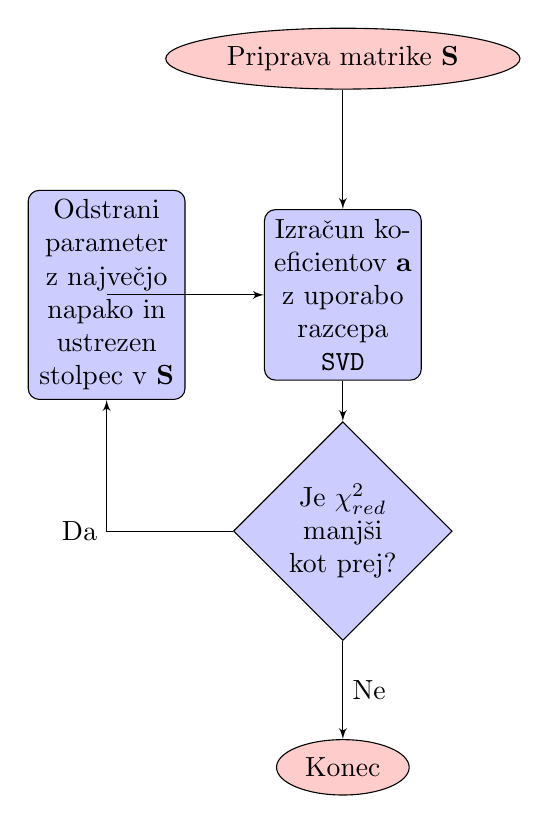
\begin{tikzpicture}[node distance = 3cm, auto]
 \node[cloud] (init) {Priprava matrike $\mathbf{S}$};
 \node[block, below of=init] (step) {Izra"cun koeficientov $\mathbf{a}$ z uporabo razcepa $\texttt{SVD}$};
 \node[decision, below of=step] (test) {Je $\chi^2_{red}$ manj"si kot prej?};
 \node[cloud, below of=test] (stop) {Konec};
  \node[block, left of=step] (remove) {Odstrani parameter z najve"cjo napako in ustrezen stolpec v $\mathbf{S}$};

\path[line] (init) -- (step);
\path[line] (step) -- (test);
\path[line] (test) -- node {Ne}(stop);
\path[line] (test) -| node {Da}(remove);
\path[line] (remove) |- (step);
\end{tikzpicture}
\caption{Shema algoritma za izlo"canje nepomembnih testnih funkcij}
\end{figure}

Ker so bili vsi moji podatk\label{fig:alg-izlocanje}
i normirani, sem lahko primerjal kar absolutne napake koeficientov, tako da sem vedno izklju"cil tistega, ki je najmanj vplival na $\chi^2$. 

\end{comment}

Preizkusil sem vse mo"zne kombinacije teh testnih funkcij, nato pa obdr"zal tisto, ki je dala najmanj"si $\chi^2_{red}$. Zaradi velikega "stevila kombinacij ($2^n$, kjer je $n$ "stevilo testnih funkcij) je bil ra"cun dolgotrajen, na sre"co pa sta razcep matrike in iskanje optimalne vrednosti parametrov hitra. V obeh nalogah sem uporabil okrog 10 testnih funkcij, v tem primeru se je ra"cun kon"cal v manj kot sekundi. 

\section{Toplotna prevodnosti}

Za testne funkcije sem uporabil nastavke oblike

\begin{align}
 \varphi_{ij} &= T^i P^j
\end{align}

kjer sta $T$ in $P$ temperatura in mo"c grelca, skalirana na interval $[-1,1]$. Ker imamo deset meritev, sem uporabil 9 testnih funkcij, tako da sta bila tako $i$ kot $j$ enaka 0, 1 ali 2. 

Izra"cun sem ponovil pri razli"cnih vrednosti konstante $\alpha$. Pripadajo"ca $\chi^2_{red}$ in optimalno "stevilo parametrov sta prikazana na grafu. 

\begin{figure}
 \input{prev-a}
  \caption{Odvisnost "stevila parameter in dobrote fita od konstante $\alpha$}
\label{fig:prev-a}
\end{figure}

Seveda je od zahtevane natan"cnosti odvisno, katera izbira za $\alpha$ je najbolj"sa. Meni osebno se je za demonstracijske namene zdela najbolj"sa izbira $\alpha \approx 1,5$, s sedmimi koeficienti in $\chi^2_{red} \approx 0,9$. S to izbiro sem izra"cunal koeficiente. Odvisnost toplotne prevodnosti od temperature in mo"ci gretja lahko sedaj zapi"semo kot

\begin{align}
 \lambda(T,P) = \sum_{i,j} a_{ij} T^i P^j
\end{align}

s koeficienti, podanimi v tabeli \ref{tab:prev}. 

\begin{table}[h]
 \centering
\begin{tabular}{|c|c|c|c|}
\hline
$i$ & $j$ & $a_{ij}$ & $\sigma_{a_{ij}}$ \\
\hline
0 & 0 & -0.42493 & 0.14529 \\
1 & 0 & -1.39982 & 0.17735 \\
2 & 0 & 0.43696 & 0.13286 \\
0 & 1 & 0 & 0\\
1 & 1 & 0.40031 & 0.15236 \\
2 & 1 & 0.16002 & 0.15608 \\
0 & 2 & 0.11553 & 0.18965 \\
1 & 2 & 0.80708 & 0.26507 \\
2 & 2 & 0 & 0 \\
\hline
\end{tabular}
\caption{Optimalne vrednosti parametrov toplotne prevodnosti}
\label{tab:prev}
\end{table}


\clearpage
\section{Teko"ci kristali}

Isti postopek sem uporabil tudi na tabelah s podatki o dol"zini disklinacij. Tokrat imamo same eno neodvisno spremenljivko, zato so bile testne funkcije kar njene potence. Za testne funkcije sem uporabil prvih 16 potenc te spremenljivke, omejil pa sem se le na kombinacije z najve"c 10 paremetri. Konstanto $\alpha$ sem zmanj"sal, ker i"s"cemo skupne "clene iz vseh treh serijah meritev, zato dopustimo ve"cje "stevilo parametrov. 


Izra"cunani parametri so v tabeli \ref{tab:wrboost}. 

\slika{kris-e}{Podatki iz datoteke \texttt{wrboost\_eight.dat}}
\slika{kris-o}{Podatki iz datoteke \texttt{wrboost\_omega.dat}}
\slika{kris-t}{Podatki iz datoteke \texttt{wrboost\_theta.dat}}

\begin{table}
 \centering
\begin{tabular}{|c|c|c|c|}
\hline
$i$ & \texttt{eight} & \texttt{omega} & \texttt{theta} \\
\hline
0 & -0.9 $\pm$ 0.1 & -0.9 $\pm$ 0.1 & -0.9 $\pm$ 0.1 \\
1 & & & \\
2 & & & \\
3 & -8.1 $\pm$ 0.5 & & \\
4 & 2.4 $\pm$ 0.4 & 1.7 $\pm$ 0.2 & \\
5 & 47 $\pm$ 2 & & \\
6 & & & \\
7 & -123 $\pm$ 6 & & \\
8 & -4 $\pm$ 1 & & 49 $\pm$ 2 \\
9 & 129 $\pm$ 7 & &  \\
10 & 3.4 $\pm$ 0.8 & & -146 $\pm$ 6 \\
11 & & & \\
12 & & & 155 $\pm$ 8 \\
13 & -91 $\pm$ 6 & & \\
14 & & & -56 $\pm$ 3 \\
15 & 44 $\pm$ 4 & & \\
\hline
$\chi^2_{red}$ & 0,21 & 0,88 & 0,20 \\
\hline

\end{tabular}
\caption{Koeficienti $a_i$ za vse tri serije meritev}
\label{tab:wrboost}
\end{table}

Izbral sem tak"sno "stevilo koeficientov, da je bil $\chi^2_{red}$ v vseh primerih pod 1. Kljub temu ni nobene testne funkcije (razen konstante), ki bi nastopala v vseh treh konfiguracijah. No podlagi teh rezultatov bi pri podani oceni napake zaklju"cil, da tak"snega "clena ni. 


\end{document}

